\documentclass[12pt,twosides,onecolumn,openany]{article}
\usepackage{graphicx} 

\usepackage{cite}
\usepackage[catalan]{babel}
\usepackage{emptypage}
\usepackage{hyperref}
\usepackage{mathtools}
\usepackage{blindtext}
\usepackage{subfigure}
\usepackage[utf8]{inputenc}
\usepackage{caption}
\usepackage{subcaption}
\usepackage{wrapfig}
\usepackage[a4paper]{geometry}
\geometry{top=2.5cm, bottom=2.5cm, left=2.5cm, right=2.5cm}
\usepackage{fancyhdr}
\pagestyle{fancy}
\usepackage{amsmath}
\usepackage{amssymb}
\usepackage{amsfonts}
\providecommand{\norm}[1]{\lVert#1\rVert}
\hypersetup{colorlinks=true,urlcolor=blue,linkcolor=blue}
\usepackage{multirow}
\usepackage{multicol}
\usepackage{rotating}

\usepackage{titlesec}

\newenvironment{Figura}
  {\par\medskip\noindent\minipage{\linewidth}}
  {\endminipage\par\medskip}

\titleformat{\section}  % comando de sección a formatear
  {\fontsize{14}{16}\bfseries} % formato para toda la línea
  {\thesection} % cómo mostrar el número
  {0.4em} % espacio entre el número y el texto
  {} % formato solo para el texto
  [] % formato para después del texto


\fancyhf{}
\fancyhead[LO,RE]{Grup D3}
\fancyhead[RO,LE]{Pràctica Ib}
\fancyfoot[LO,RE]{\thepage}
\fancyfoot[RO,LE]{Laboratori de Termodinàmica - UAB}
\graphicspath{ {images/} }

\begin{document}

\begin{center}
    {\Large \textsc{Transport de la calor: Comprovació de la llei de Stefan}}\\
    \vspace{0.2cm}
    \textsc{30 d'Octubre de 2024}\\
    \vspace{0.2cm}
    $\begin{matrix} 
    \text{Miguel A.} \hspace{1.5cm} & \text{Daniel B.} & \hspace{1.5cm} \text{Sergi R.}\\1637738 \hspace{1.5cm} & 1603508 & \hspace{1.5cm} 1607805
    \end{matrix}$
\end{center}
\begin{center}
    \textsc{\textit{RESUM}}
\end{center}
Lorem ipsum dolor sit amet, consectetur adipiscing elit, sed do eiusmod tempor incididunt ut labore et dolore magna aliqua. Ut enim ad minim veniam, quis nostrud exercitation ullamco laboris nisi ut aliquip ex ea commodo consequat. Duis aute irure dolor in reprehenderit in voluptate velit esse cillum dolore eu fugiat nulla pariatur. Excepteur sint occaecat cupidatat non proident, sunt in culpa qui officia deserunt mollit anim id est laborum.
\vspace{0.5cm}
\begin{multicols}{2}
\section{Introducció i objectius}
\begin{equation}\label{Llei_Ohm}
  V =IR
\end{equation}
\begin{equation}\label{Pot_elec}
  P_{\text{e}} = VI
\end{equation}
\begin{equation}\label{Newton}
  P_{\text{c}} = -\lambda A\Delta T
\end{equation}
on $\Delta T = T - T_a$ 
\begin{equation}\label{ln_Newton}
  \ln{P_{\text{c}}} = \ln{\Delta T} + \ln{(-\lambda A)}
\end{equation}
\begin{equation}\label{Stefan_Boltzmann}
  P_{\text{r}} = e\sigma_{\text{SB}}AT^{4}
\end{equation}
\begin{equation}\label{relacions_pot}
  P_{\text{e}}=P_{\text{c}} + P_{\text{r}}
\end{equation}
\begin{equation}\label{resistencia}
  R = R_0[1+\alpha\Delta T]
\end{equation}
\section{Resultats i discussió}
A partir de les dades experimentals recollides obtenim la Figura \ref{fig:lnP_vs_lnDeltaT}.
\begin{Figura}
  \centering
  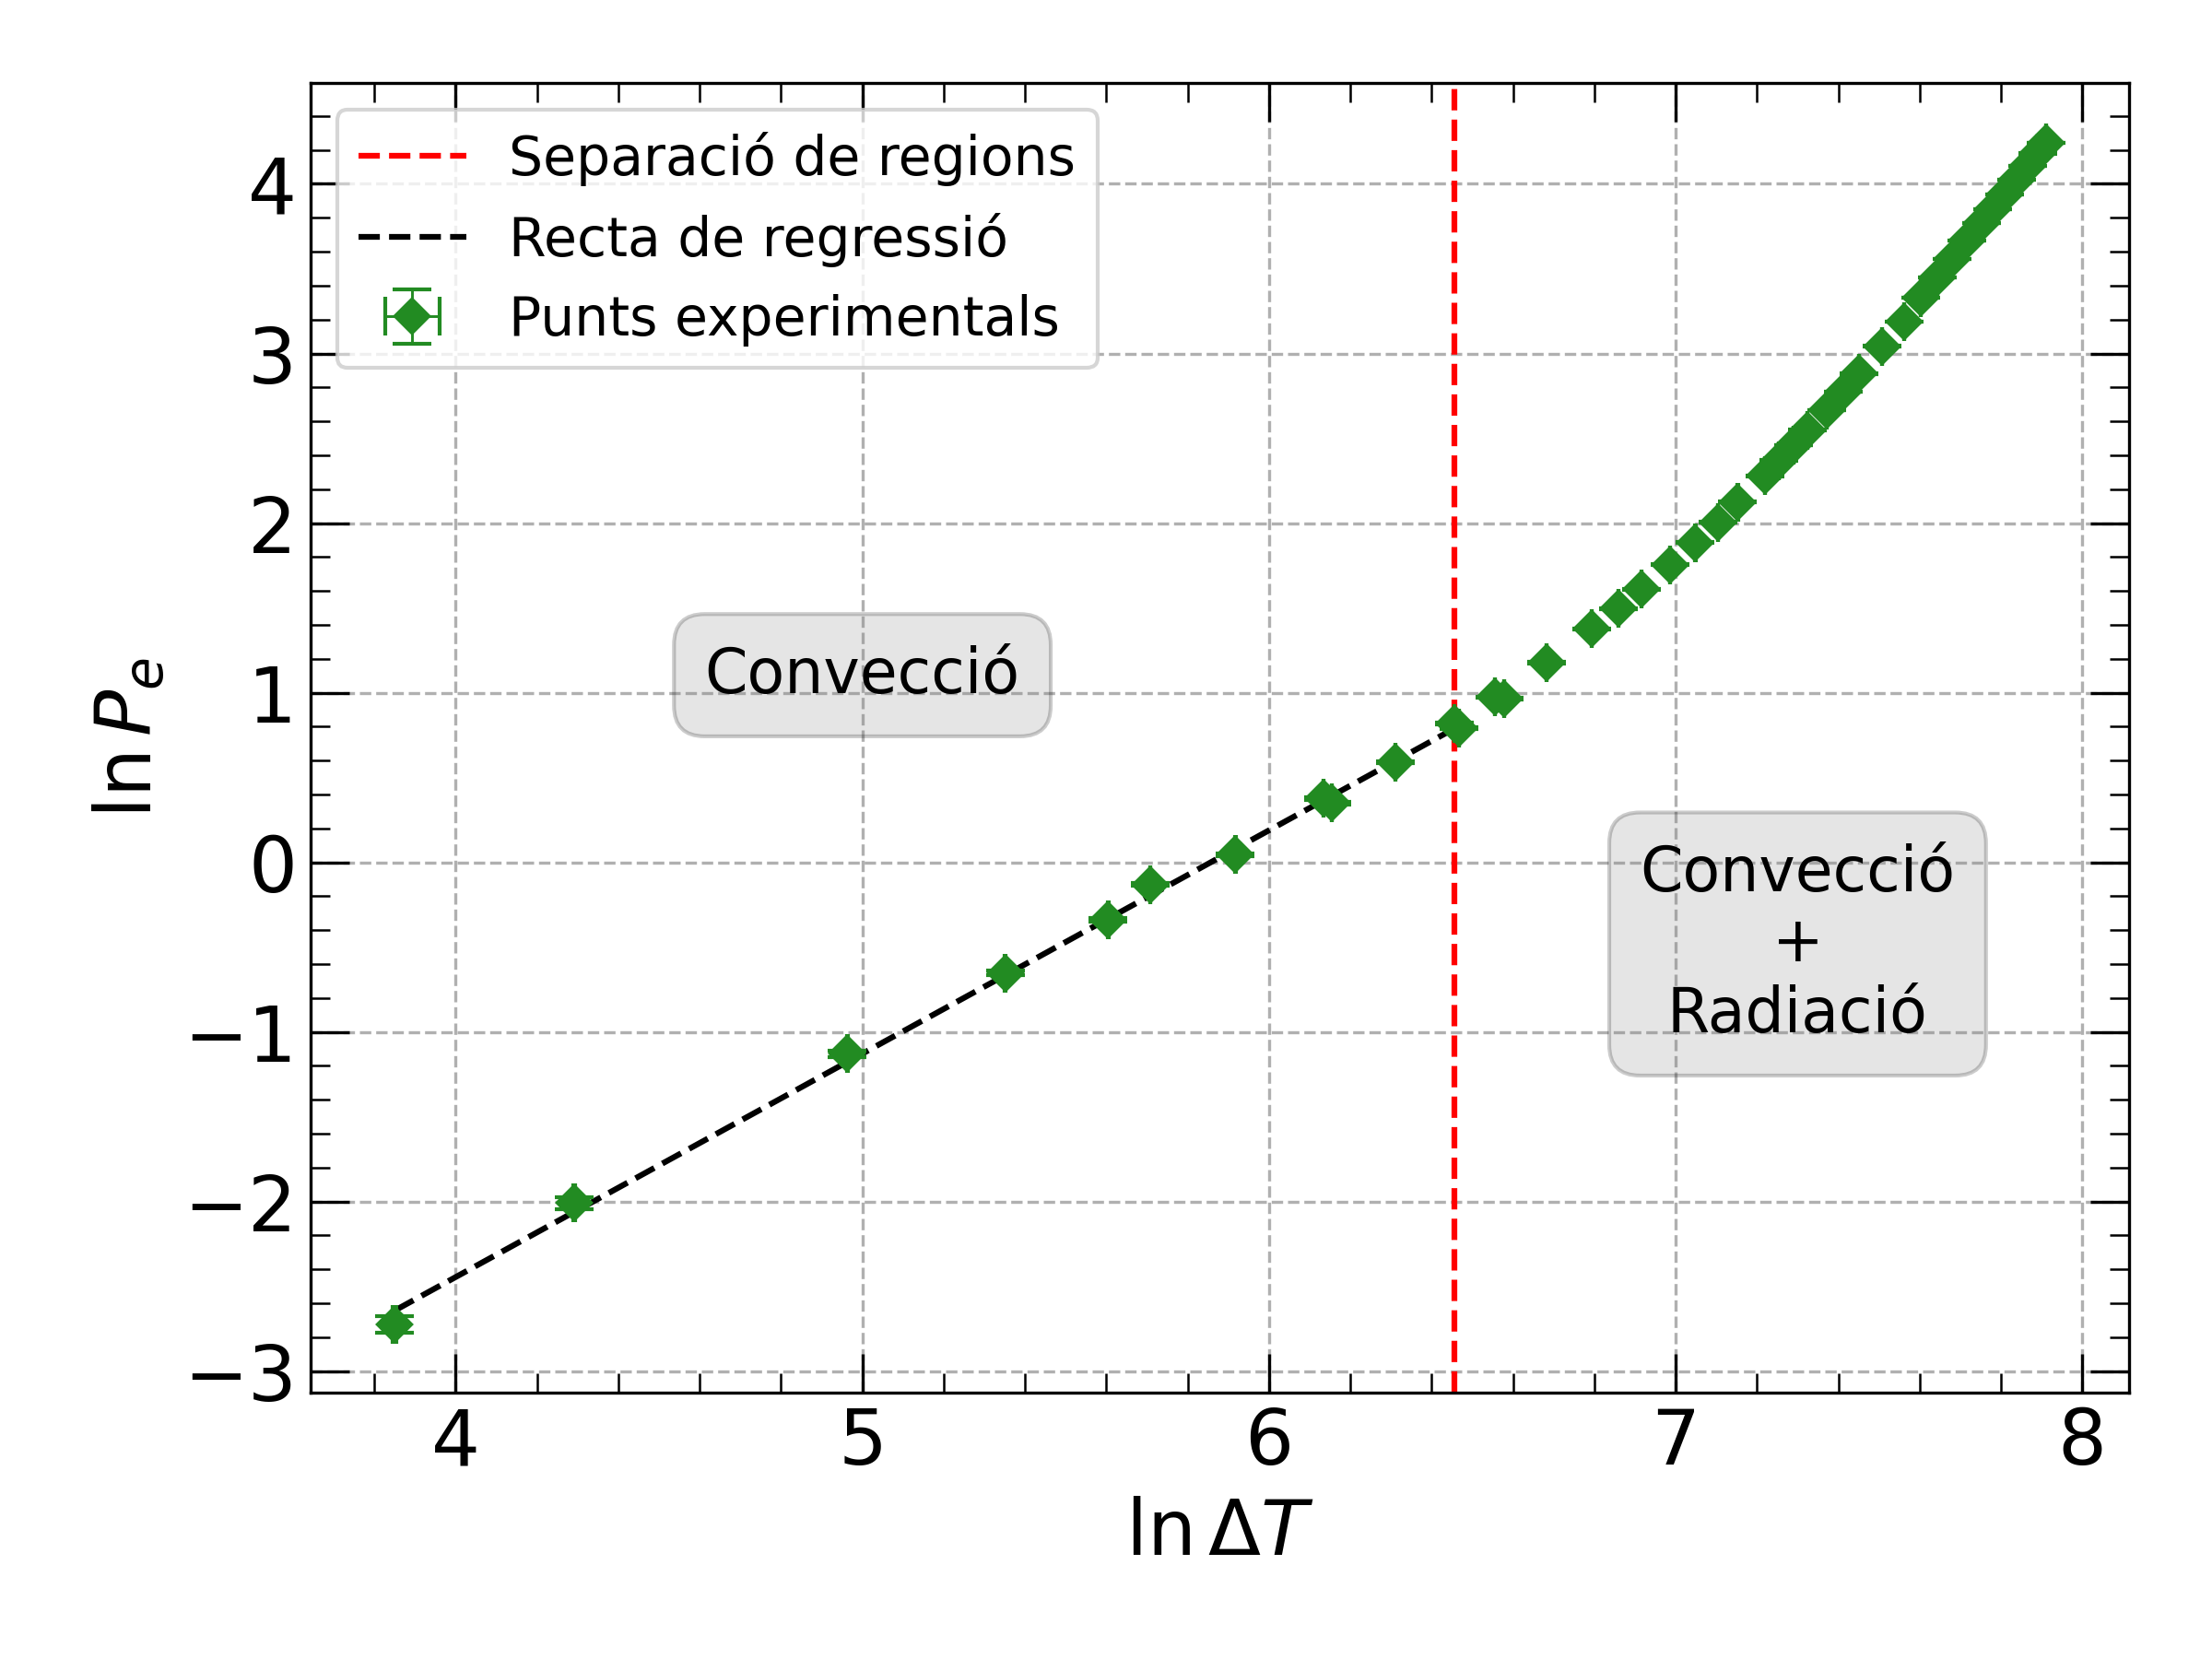
\includegraphics[width=\linewidth]{../../graphs/practica_Ib/plots/lnP_el_vs_lnT.png}
  \captionof{figure}{\footnotesize{Gràfica $\ln{P}$ vs $\ln{\Delta T}$.}}
  \label{fig:lnP_vs_lnDeltaT}
\end{Figura}
S'observen dues zones diferents, una amb comportament lineal i una altra amb un comportament diferent. Agafant punt a punt i de forma ordenada (de $\Delta T$ menor a major) valors experimentals repressentats a la Figura \ref{fig:lnP_vs_lnDeltaT} fem diverses regressions lineals de forma iterada fins a obtenir el major valor per al coeficient de regressió $r^2$, obtenint el valor 11 com a nombre òptim de punts. Es pot veure repressentada a la mateixa Figura \ref{fig:lnP_vs_lnDeltaT} la regressió lineal obtinguda amb la llista de punts resultants. S'observa a la Taula \ref{tau:reg_lnP_vs_lnDeltaT_part1} els valors d'aquesta regressió.
\begin{Figura}
  \centering
  \captionof{table}{\footnotesize{Valors de regressió de la part de convecció lnp vs lnDeltaT}}
  \begin{tabular}{c|c}
    \hline \hline
    $m$ & $b$ \\
    \hline
    $1,317 \pm 0,017$ & $-7,712\pm0,097$\\
    \hline \hline
  \end{tabular}
  \label{tau:reg_lnP_vs_lnDeltaT_part1}
\end{Figura}
Com es pot observar a l'Equació \eqref{ln_Newton} el pendent d'aquesta regressió hauria de ser $m=1$ si al sistema només s'intercanviés calor per convecció. Però,les dades obtingudes porten a deduir que aquesta hipòtesi inicial és incorrecta, és a dir, tot i ser petita, existeix una contribució de calor per radiació.\\\\
Tenint en compte l'Equació \eqref{relacions_pot} podem calcular a la segona regió marcada a la Figura \ref{fig:lnP_vs_lnDeltaT} restant als valors experimentals la contribució per convecció. Per a fer això podem, a partir de les dades de regressió de la Taula \ref{tau:reg_lnP_vs_lnDeltaT_part1}, extrapolar els punts necessaris i fer la resta. Podem observar amb més detall la segona regió i la extrapolació a la Figura \ref{extrapolacio}.
\begin{Figura}
  \centering
  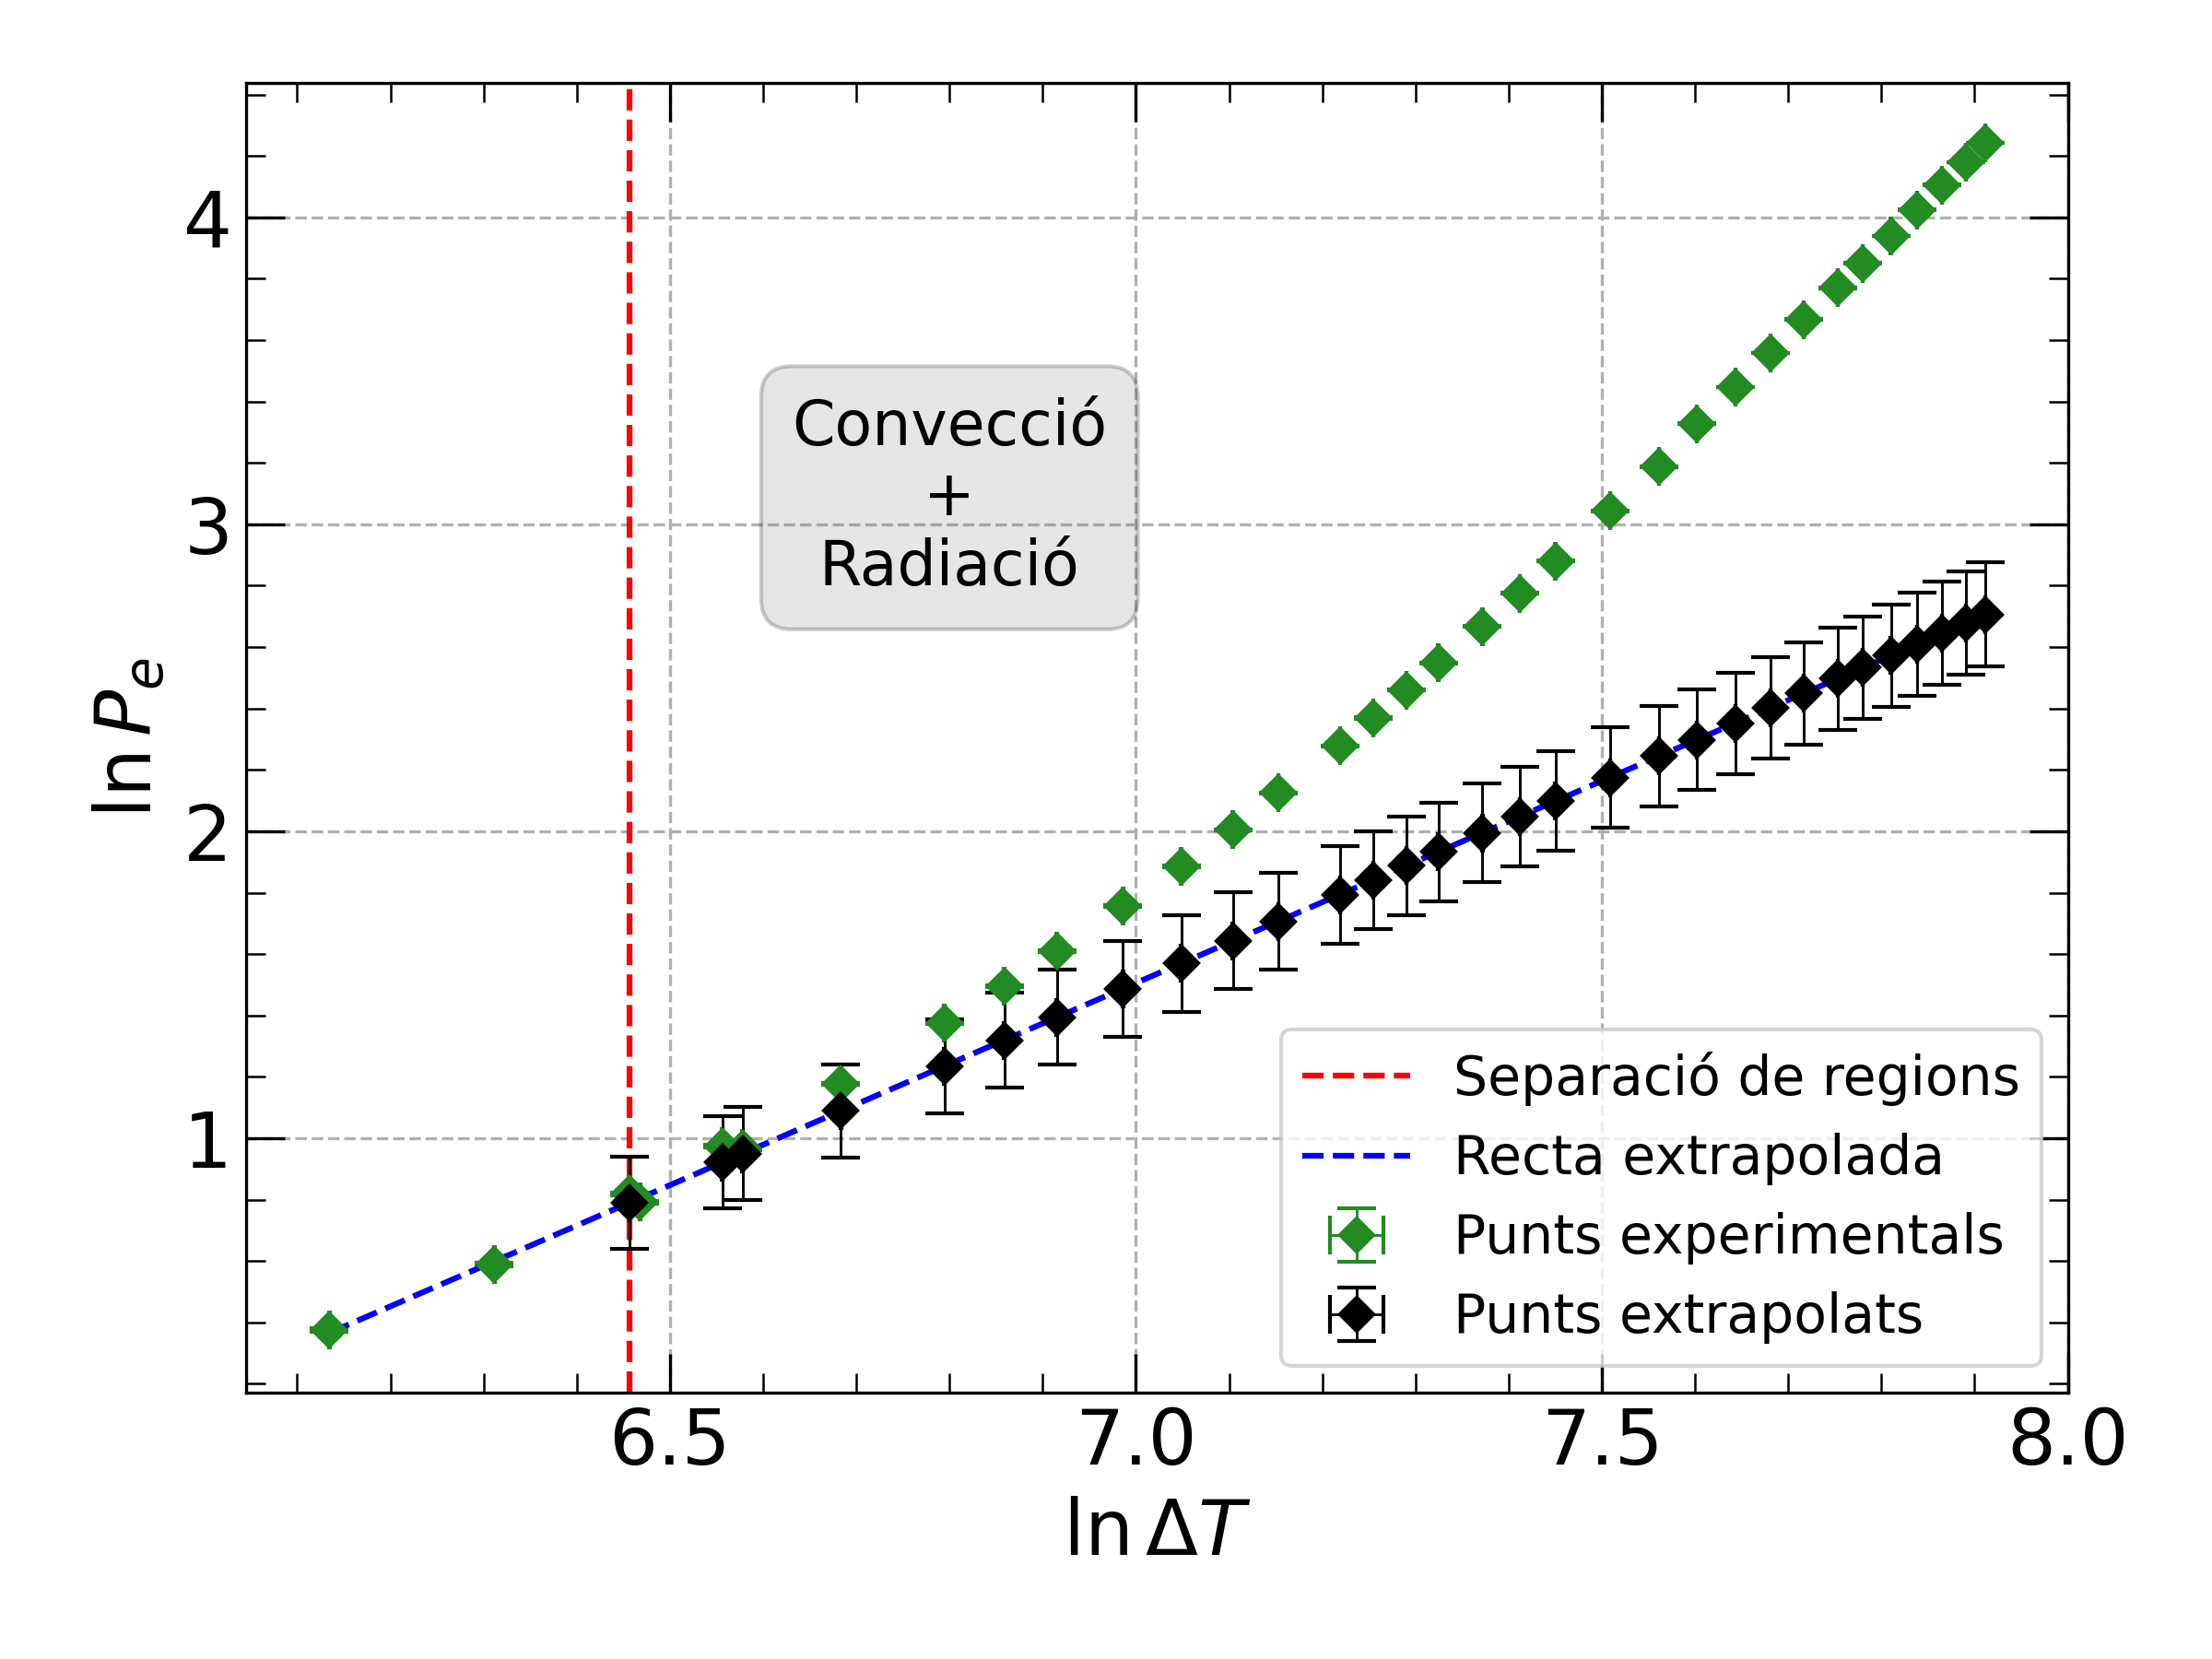
\includegraphics[width=\linewidth]{../../graphs/practica_Ib/plots/extrapolació.png}
  \captionof{figure}{\footnotesize{Ampliació gràfica i recta de extrpolació.}}
  \label{extrapolacio}
\end{Figura}
Aamb aquest conjunt de dades $\ln{P_{\text{e}}}$ i $\ln{P_{\text{c}}}$ a la regió de la dreta recalculem els valors $P_{\text{e}}$ i $P_{\text{c}}$ corresponents i apliquem l'Equació \eqref{relacions_pot}. Amb el resultat tornem a graficar els logaritmes, obtenint la Figura \ref{fig:lnP_rad_vs_lnDeltaT}
\begin{Figura}
  \centering
  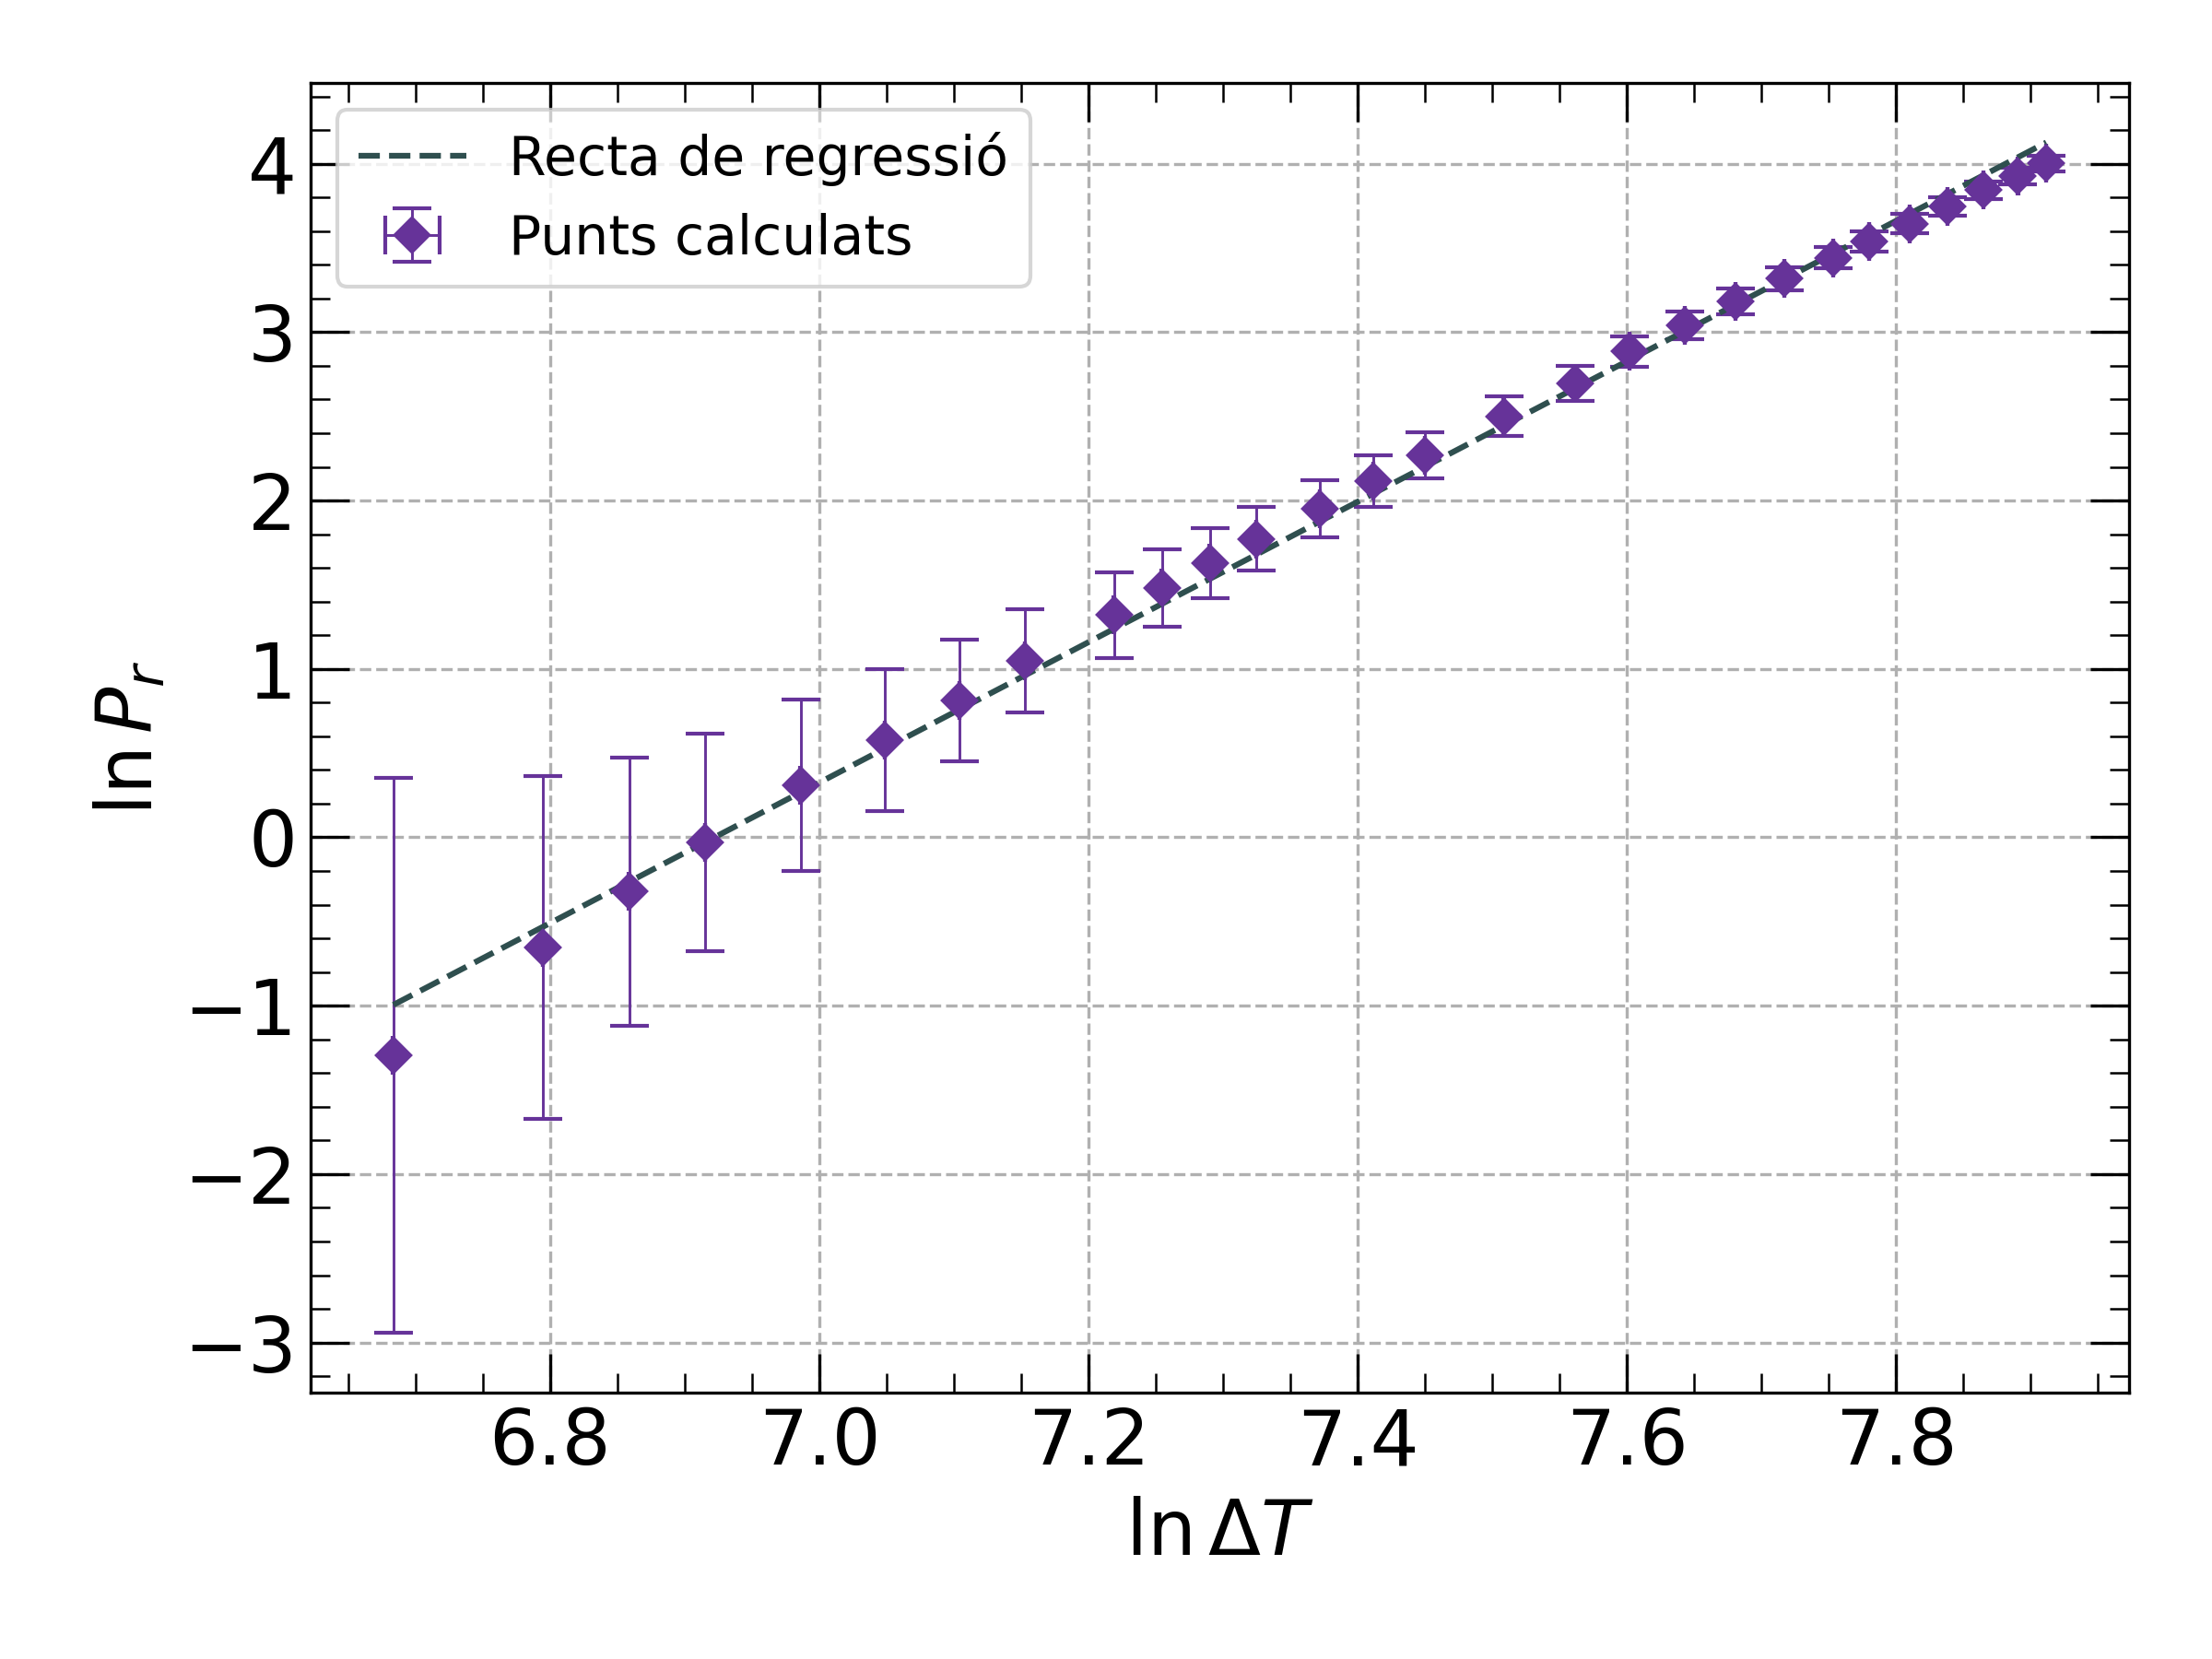
\includegraphics[width=\linewidth]{../../graphs/practica_Ib/plots/lnp_rad_vs_lnDelta_T.png}
  \captionof{figure}{\footnotesize{Logaritme de log(Prad) vs log(DeltaT)}}
\end{Figura}
\section{Conclusions}
\section{Annex}
\end{multicols}
\end{document}